%%
%% Berliner Hochschule für Technik --  Abschlussarbeit
%%
%% Kapitel 2
%%
%%

\chapter{Zweiter Abschnitt}\label{ch.test}

In diesem Abschnitt folgt reichlich Blindtext, um das Aussehen voller Seiten zu
dokumentieren. 

\section{Grundlegendes}

\begin{neu}
  \blindtext \anno{Sachen gibt's!}
\end{neu}
\blindtext 

\section{Weiterführendes} 

\begin{neu}
  \blindtext
\end{neu}

\blindtext
\blindenumerate
\blindtext[3] \anno{Lesen, bitte!}

\begin{figure}[bht]
  \begin{center}
    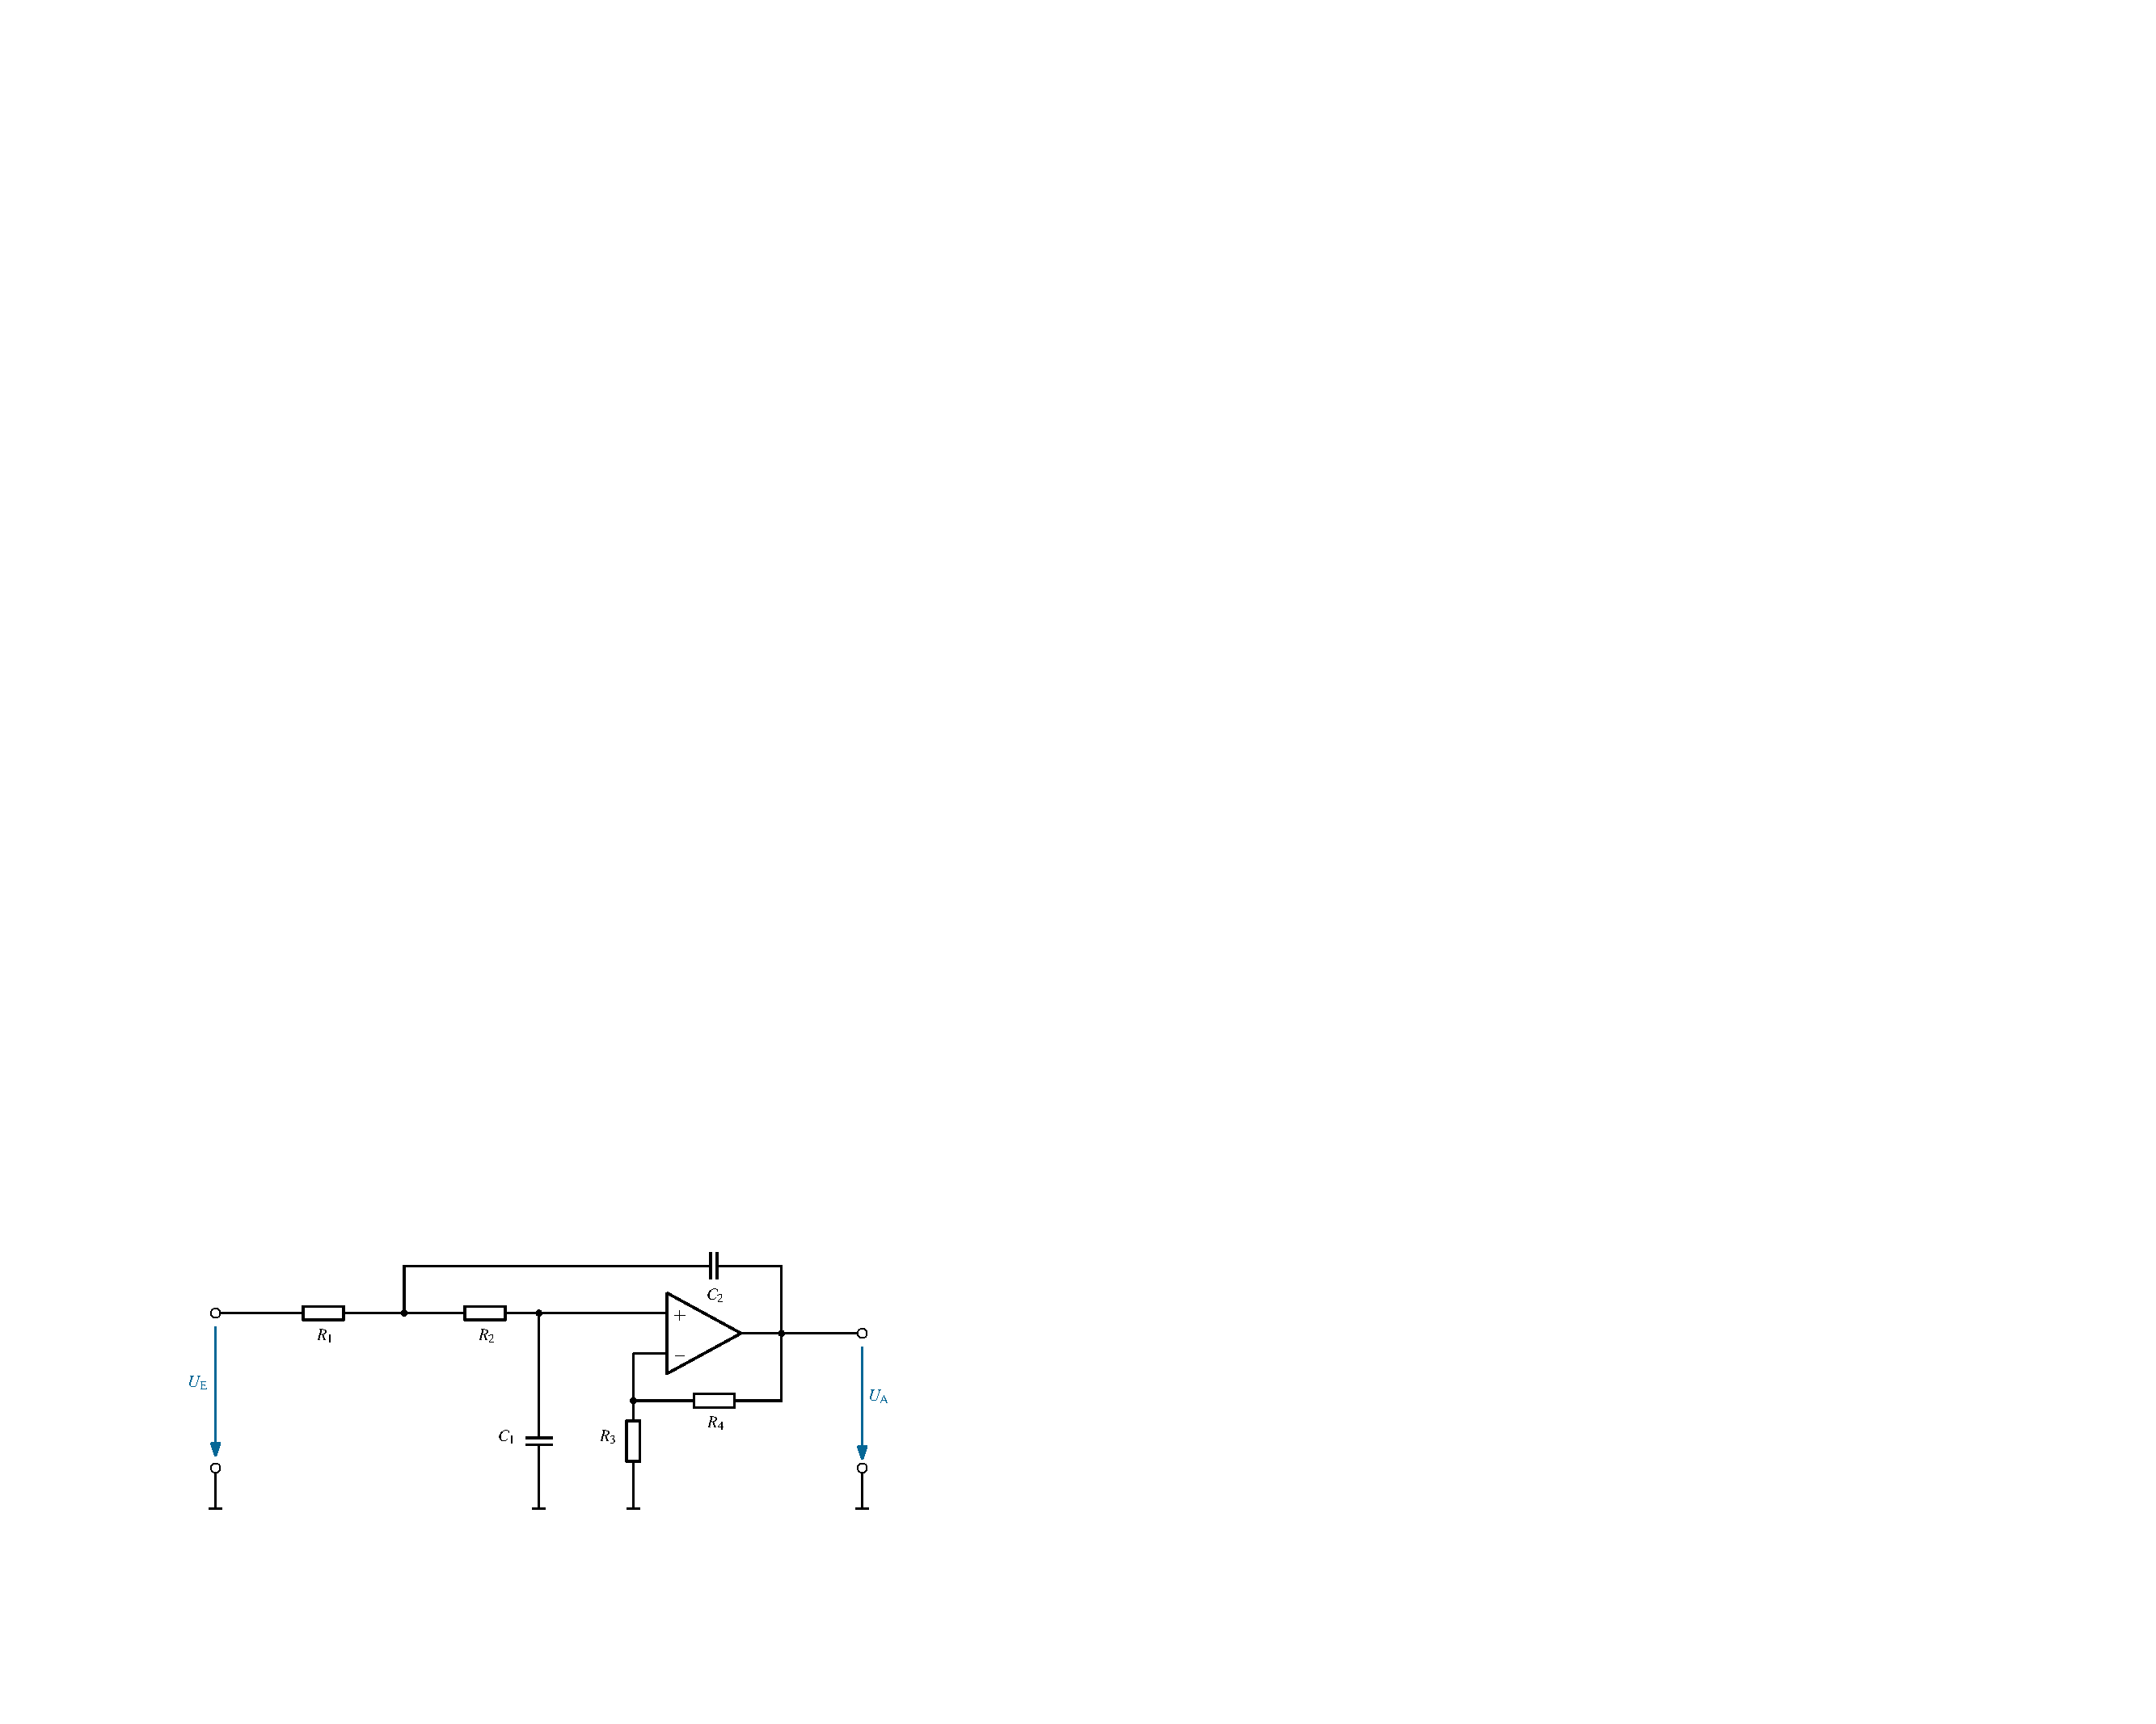
\includegraphics[scale=1]{schaltbild}
    \caption{Die verwendete Filterschaltung}
    \label{fig.Filterschaltung}
  \end{center}
\end{figure}

\blinditemize[8]
\Blindtext[2][2]
\blinddescription \anno{Es ist auch möglich längere Randnotizen zu machen. Ob die 
  dann aber gelesen werden, ist so eine Sache}  

\section{Abwegiges}

\blindtext

